\chapter{From edges to contours} % - Current State-of-the-Art}
\label{Chapter3}
\settocdepth{subsubsection}

In this chapter we review a recent segmentation method, introduced in \cite{Arbelaez09} and further developed %refined 
in \cite{Arbelaez11}.

\begin{figure}[ht!]
\centering
 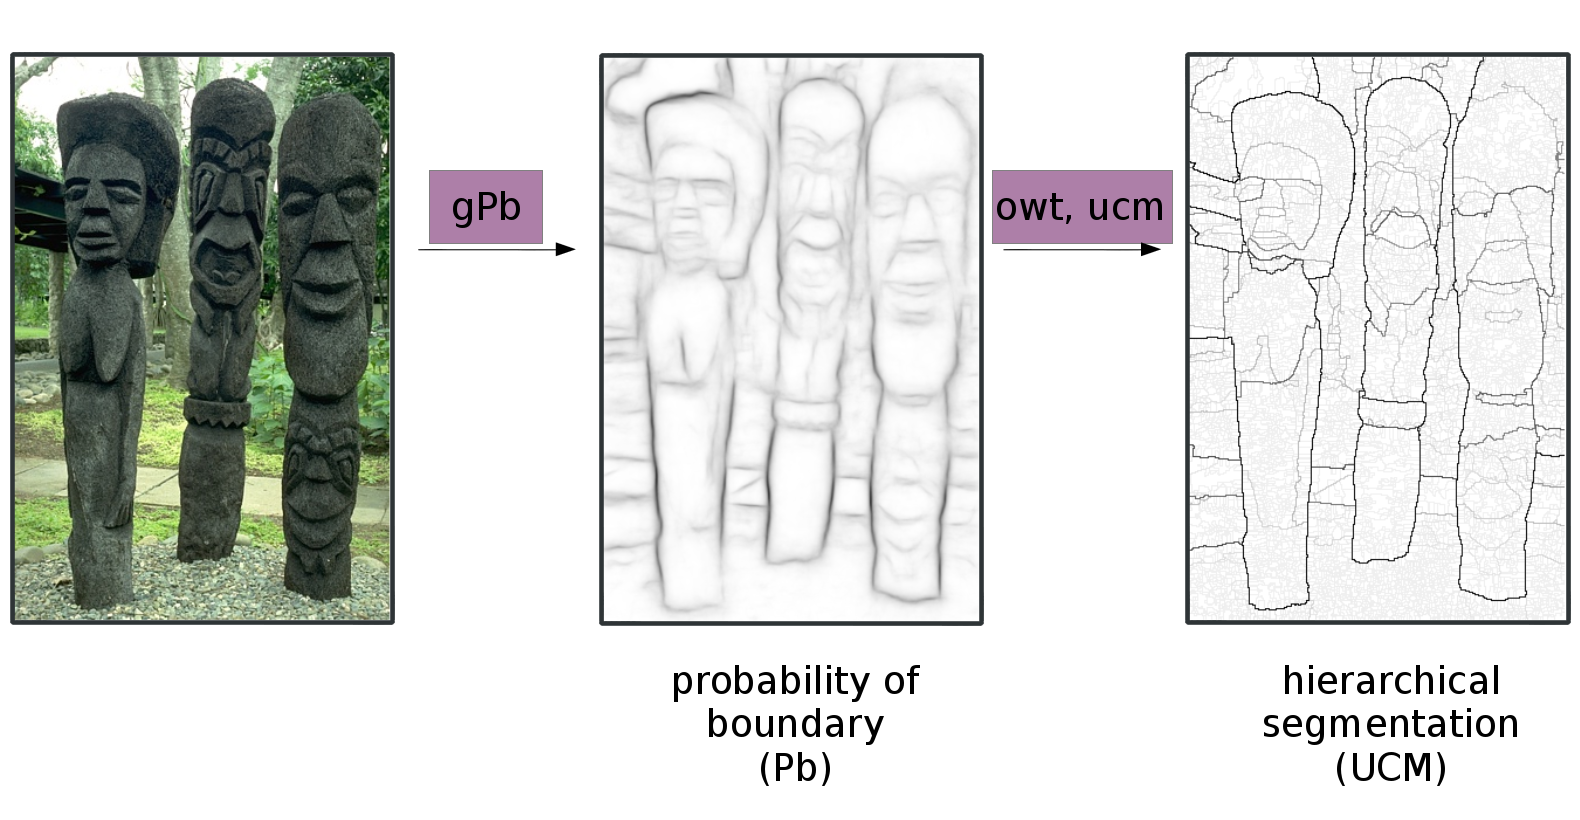
\includegraphics[width=1\textwidth]{images/gPb-OWT-UCM/gPb-OWT-UCM-high-level.png}
\caption[High-level view of gPb-OWT-UCM algorithm]{High-level view of gPb-OWT-UCM - a segmenter that extracts edges and uses them to obtain a multiscale segmentation.}
\label{fig:gPb-OWT-UCM-high-level}
\end{figure}


\section{gPb-OWT-UCM algorithm pipeline}
\begin{figure}[ht!]
\centering
 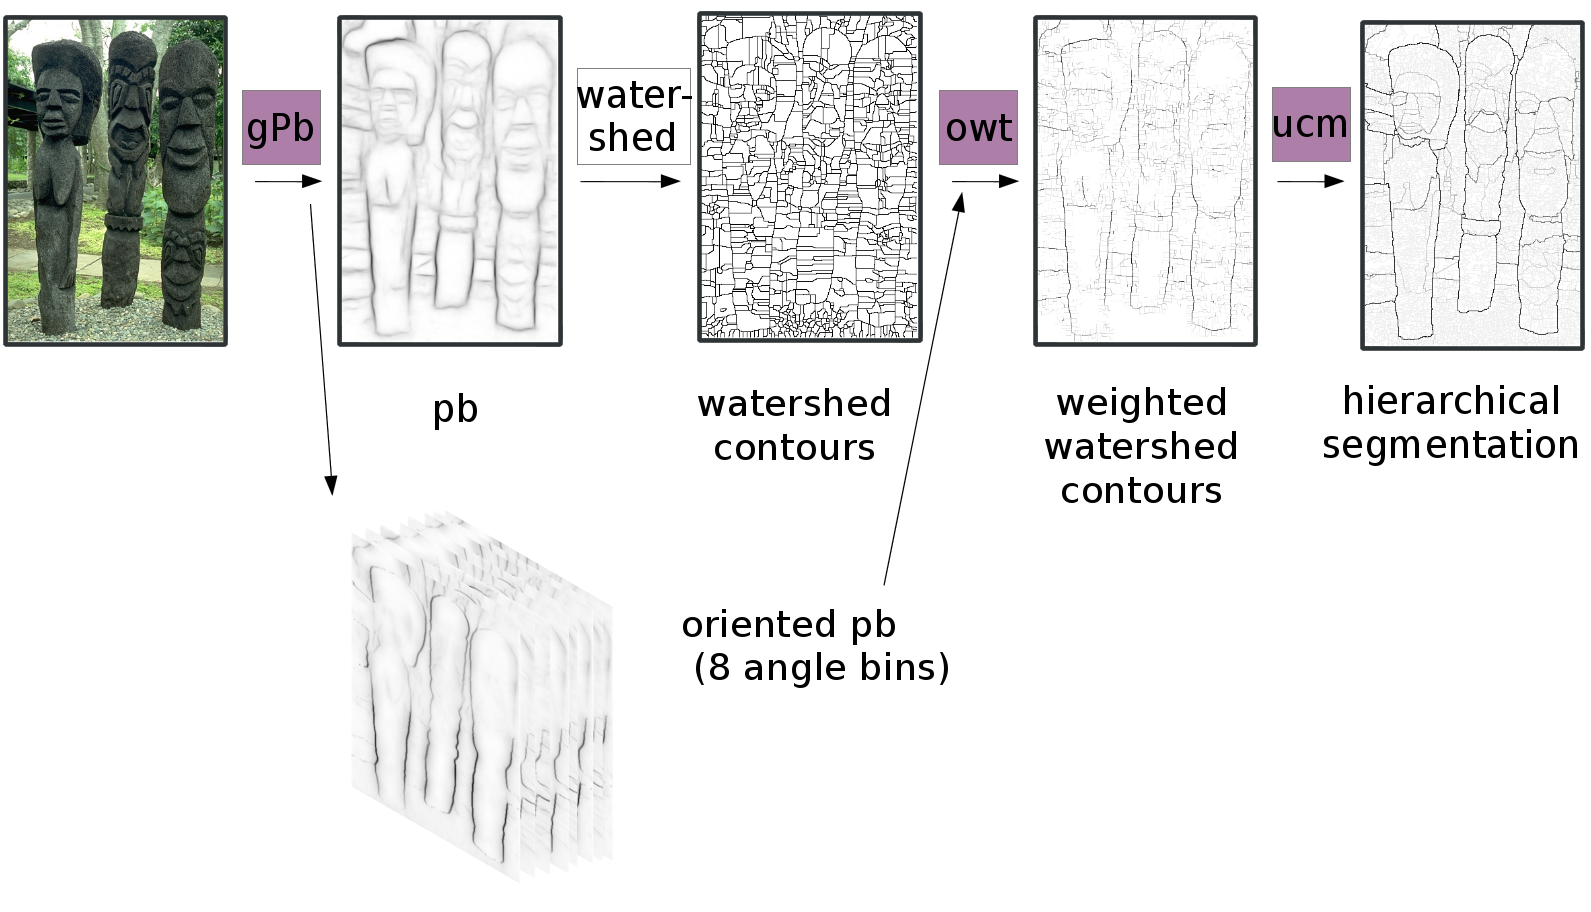
\includegraphics[width=1\textwidth]{images/gPb-OWT-UCM/gPb-OWT-UCM_pipeline.png}
\caption[gPb-OWT-UCM algorithm detailed pipeline]{gPb-OWT-UCM detailed algorithm pipeline. We are explicitly including the ``watershed transform'' operation and its output - watershed contours, as it is cruicial both to this technique and our method, which we propose in \cref{Chapter4}.}
\label{fig:gPb-OWT-UCM-pipeline}
\end{figure}

\subsection{First stage of the pipeline - edge detection} % gPb
\label{sec:ch3-gPb}
The gPb algorithm utilises local cues - colour, brightness and texture to build features. Those are then globalised using spectral clustering. Multiple-scale approach gives competitive edge detection results.
% TODO discuss multiple orientations; put image
% TODO effective cue combination!

Coarse-to-fine is a powerful concept in computer vision \cite{Ren2008multi}. It is employed in the mPb part of the edge detector to allow to capture the salient edges at different scales.
% mPb fires at all edges, sPb fires at salient edges => combine lienarly (learn the weight)

\textbf{Quantised oriented probability of boundary}
\subsection{Second stage of the pipeline - weighting the watershed} % OWT
The idea for the last two phases of the pipeline is that weighted watershed contours can be converted into a hierarchical segmentation.

\subsubsection{Watershed}
\label{sec:ch3-watershed}
% TODO
% from Marco's blog
%- The Watershed transformation considers the gradient magnitude of an image as a topographic surface. Pixels having the highest gradient magnitude intensities (GMIs) correspond to watershed lines, which represent the region boundaries. Water placed on any pixel enclosed by a common watershed line flows downhill to a common local intensity minima (LMI). Pixels draining to a common minimum form a catchment basin, which represent the regions.

%- The figure below depicts how the regions are found. (a) is a matrix showing typical GMI values with the LMIs circled. (b) shows the morphological gradient directions for the matrix in (a).

%- A major problem with this method is that it very often results in severe over segmentation, such as in the segmentation below. There have been several attempts at overcoming this problem. Meyer and Beucher proposed a marker-controlled strategy. Markers are placed on the image to represent objects. The Watershed transformation is then run by flooding from the markers. This requires prior knowledge of the objects in the image or even manual input.
\fref{fig:watershed-transformation-forming-regions}

\begin{figure}[ht!]
 \centering
 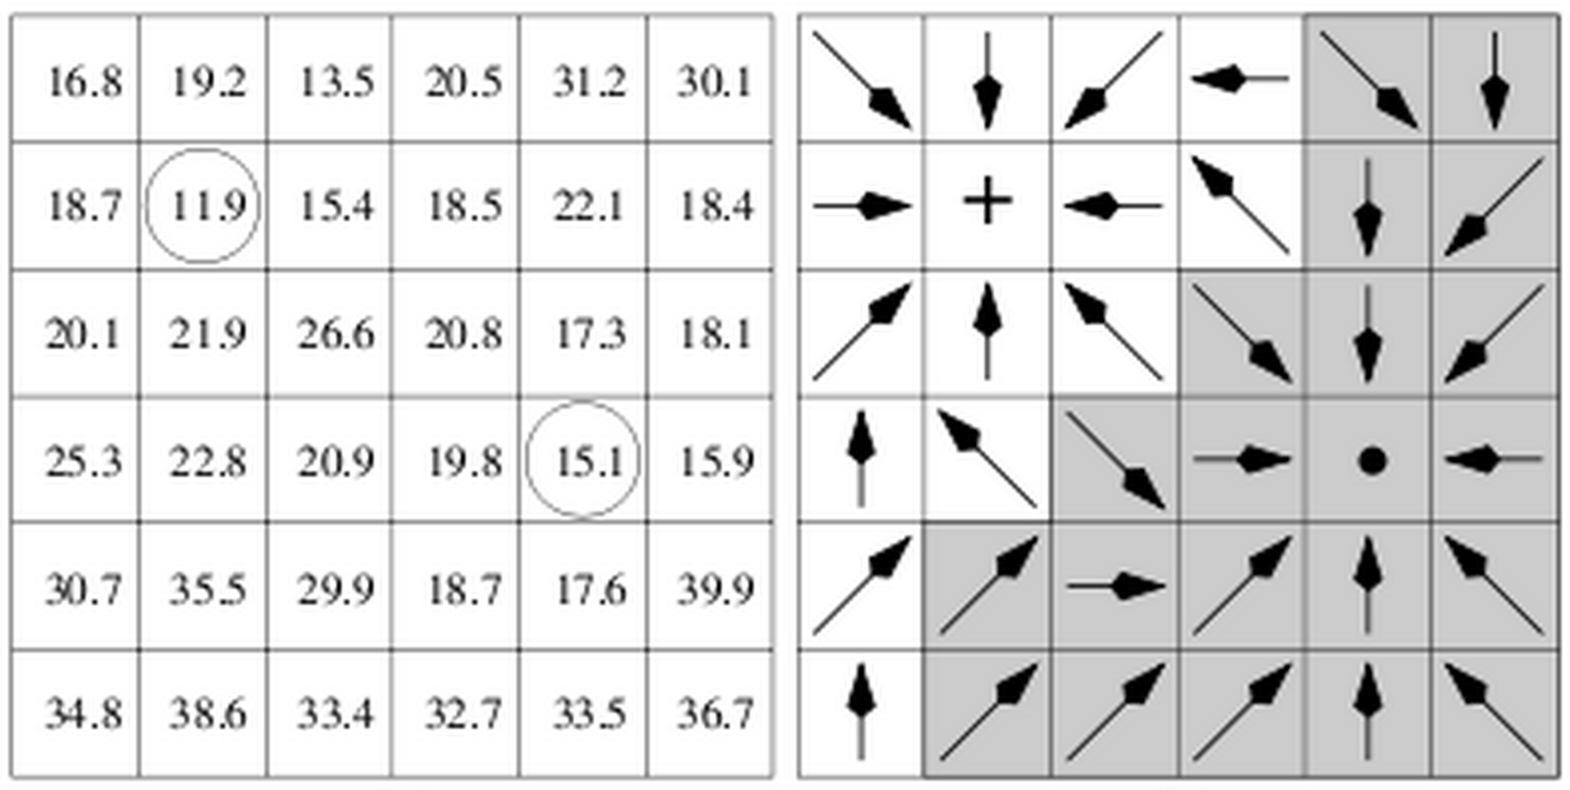
\includegraphics[width=0.5\textwidth]{images/gPb-OWT-UCM/watershed-transformation-forming-regions.png}
 \caption[Watershed transformation - forming the regions]{Watershed transformation - forming the regions. Courtesy of \cite{MarcoBlog2007Watershed}.}
 \label{fig:watershed-transformation-forming-regions}
\end{figure}

% The watershed transform is a basic morphological operation \cite{Beucher1992morphological} used to produce an image segmentation. 
Given an intensity %a greyscale 
image as an input, it would output watershed \textit{segments} (\textit{regions}), which are complimentary to the watershed \textit{pixels} (\textit{contours}). The latter are by construction closed contours. A well-known shortcoming of the watershed transform is that the 
segmentation produced by it is an oversegmentation, due to a catchment basin forming around every regional minimum.

Unlike ``Seeded region growing'' \cite{Adams1994seeded}, the watershed algorithm does not require as input any initial seeds for forming watershed regions.

Note that the watershed algorithm only provides a single segmentation, but does not build a hierarchy. %but not weights to them, hence, 
Najman~\etal \cite{Najman1996geodesic} offer a way to obtain a hierarchy of segmentations from the watershed pixels, which unfortunatelly involves the selection of a set of markers.

The watershed transform is a suitable intermediate step in obtaining hierarchical segmentation from edge detection output, since it provides a straightforward means to close contours. The probability of boundary is a one-channel image and can therefore be used as an input to the watershed transform. Thus, the locations of the watershed contours constitute a binary image indicating the higest level of recall in the context of the Precision-Recall framework of~\cite{Arbelaez11}. % (c.f. edge map)

In practice the vanilla watershed implementation in MATLAB \cite{MATLABwatershed} is used, with 8-connected neighbourhood for the regions.

\settocdepth{section}
\subsubsection{Oriented watershed transform (OWT)}
\settocdepth{subsubsection}
\label{sec:ch3-OWT}
\paragraph{Watershed arc}\mbox{}\\\mbox{}\\
\label{par:ch3-watershed-arc}
\subparagraph{Subdivision of edges}\mbox{}\\\mbox{}\\
Maire \etal \cite{Maire2008using} applied the idea of an approximation %of a boundary 
with a line first to {\bf edges} in order to facilitate localisation of junctions (and thus ``close'' contours). \fref{fig:Maire08using-contour-subdivision} shows a few edge fragments in a local image patch and (overlaid) their {\it line segment} approximations.

\begin{figure}[ht!]
 \centering
 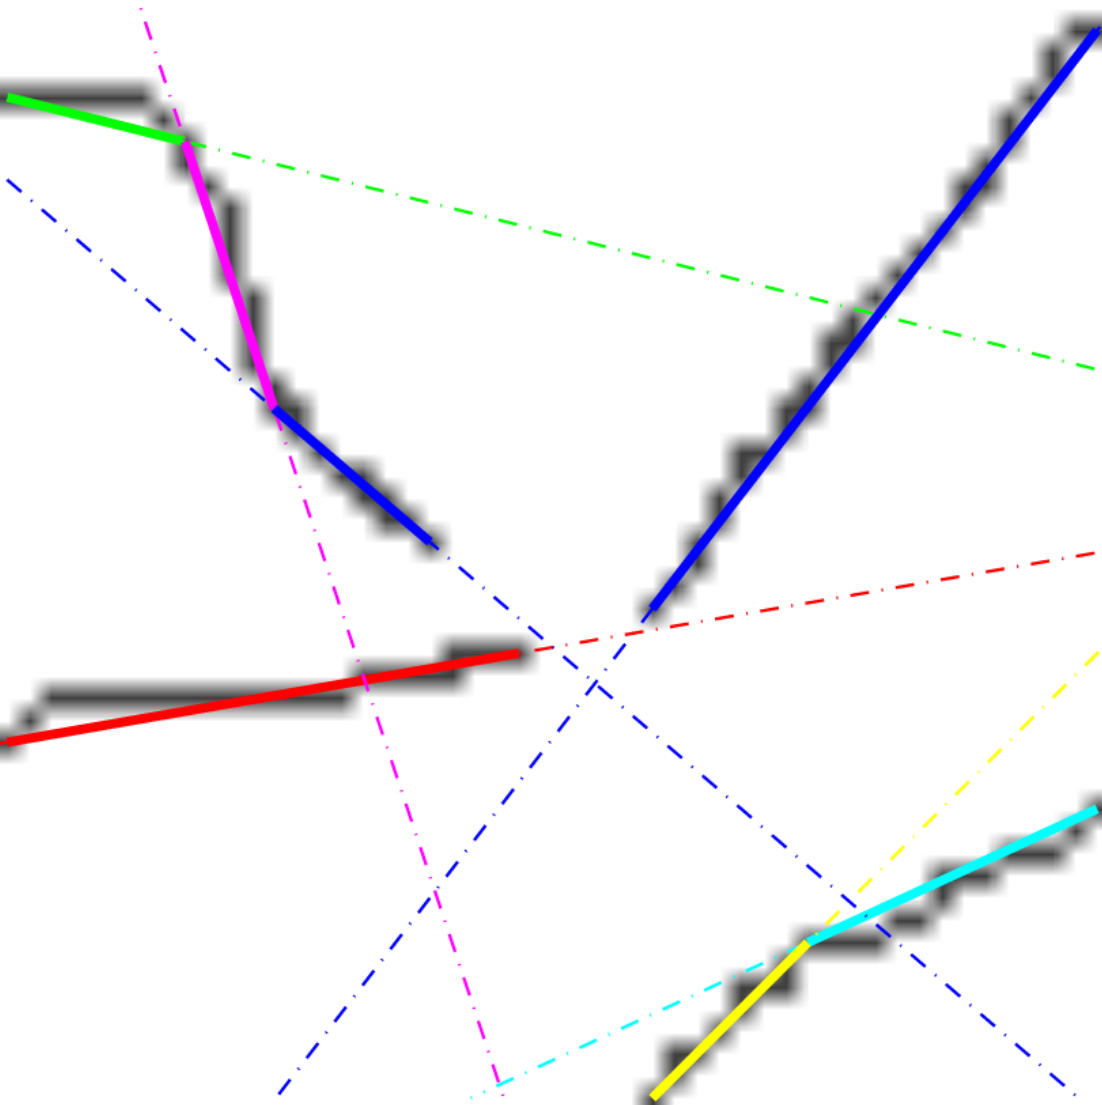
\includegraphics[width=0.4\textwidth,frame]{images/gPb-OWT-UCM/Maire2008using-contour-subdivision.png}
 \caption[Edges subdivision - an image patch]{{\bf Edges subdivision} into approximating linear pieces (solid line segments). The underlying straight lines (dashed and dotted line) would serve for junction detection. Courtesy of~\cite{Maire2008using}.}
 \label{fig:Maire08using-contour-subdivision}
\end{figure}

\subparagraph{Subdivision of region boundaries}\mbox{}\\\mbox{}\\
This scheme is easily transferable to {\bf watershed contours}. The procedure is as first described in ``From contours to regions: An empirical evaluation'' \cite{Arbelaez09}. The {\bf watershed arcs} are recursively subdivided boundaries of watershed regions. An arc is split at an internal point which is maximally distant from the straight line through % connecting 
its endpoints. The {\it subdivision} is scale-invariant: the process stops when the maximal distance from an arc point to the {\it line segment} approximating it becomes smaller than a fixed fraction of the latter's % its %the segment's 
length. See also \fref{fig:Arbelaez11-contour-subdivision}.

\begin{figure}[ht!]
 \centering
 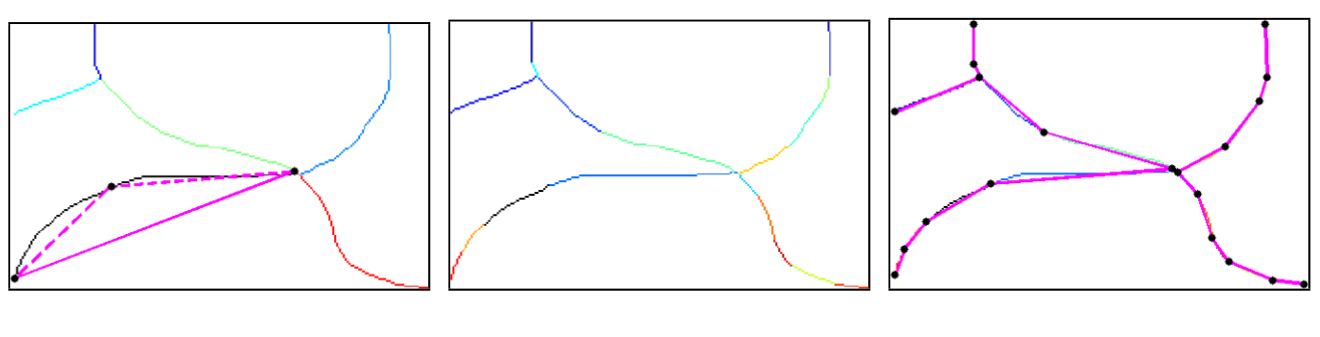
\includegraphics[width=1\textwidth]{images/gPb-OWT-UCM/Arbelaez11-contour-subdivision.png}
 \caption[Region boundary subdivision]{{\bf Region boundary subdivision} (courtesy of~\cite{Arbelaez11}). {\bf Left:} Colour-coded are given the initial watershed arcs - the full region boundaries. Magenta solid line denotes the line approximation to the arc. A subdivision (to the farthest point on the arc) is indicated with two magenta dashed lines. {\bf Middle:} The final set of watershed arcs. A region boundary consists therefore of one or more arcs. {\bf Right:} The middle image, with the arc-approximating lines (magenta solid) overlaid.}
 \label{fig:Arbelaez11-contour-subdivision}
\end{figure}

\subsection{Third stage of the pipeline - UCM}
\label{sec:ch3-UCM}
The {\it Ultrametric contour map} (UCM) was introduced in \cite{Arbelaez2006boundary}. It constitutes a convenient data structure for the representation of a hierarchical segmentation, as we hinted in the introductory \cref{Chapter1}. 

The map is constructed by agglomerative clustering of regions based on the weight of their common boundary. It represents a tree, at the leaves of which are the superpixels at the highest level of detail. Going up the tree merges regions. It is a real-valued image (see \fref{fig:sub:segmentation-ucm} and \fref{fig:sub:segmentation-ucm-cc}) in which every region boundary is weighted by its scale of disappearance.

% TODO

% Multiple segmentatons, but going up the UCM coarsens the segmentation.

% TODO give the algorithm in an appendix

\section{Limitations of the gPb-OWT-UCM} %quantisation} % or drawbacks, don't say 'flaws'
\textbf{Low speed at test time:} One undeniable % undoubted, unquestionable, indisputable
limitation of the gPb-OWT-UCM method is that it is slow on detection. On the BSDS500 dataset the segmenter takes on average 200 seconds per image.

\textbf{Quantisation:} Another issue has mostly to do with the concept of using quantisation per angle orientation to estimate strength of boundary, as well as weights for the pixels on the watershed controus. It is a crude substitute for an actual edge and therefore, incapable of capturing fine variations in the boundary shape.

\textbf{OWT-UCM not convenient for general segmentation based on edge detection:} The algorithm is in essence an elaborate pipeline that does not easily accomodate different edge detectors. It has as an intrinsic ingredient the oriented probability of boundary. Nevertheless, many algorithms (\eg \cite{Kisilev2013Learning,Arbelaez2014multiscale,Isola2014crisp,Hallman2014}) re-use the second and third stage of the gPb-OWT-UCM pipeline to also obtain segmentation in addition to their extracted esges.

In \cref{Chapter4} we propose a more coherent % logical and consistent
and principled approach, which has the potential of addressing the above issues. It makes use of the detailed structured information present in local edge image patches. By applying this local knowledge it dispenses with the computation of oriented gradient signals for a fix number of orientations that is prevalent in the gPb-OWT-UCM pipeline.
